% ==========================================================================
% INFO 4617 Web Data Science -- Week 11: Government Data APIs (Chapter 11)
% Build:  TEXINPUTS=../common: BIBINPUTS=../common: latexmk -pdf slides.tex
% (or run `make` from the slides/ directory)
% ==========================================================================
\documentclass[9pt,aspectratio=169]{beamer}
% ==========================================================================
% Shared preamble for INFO 4617 Web Data Science weekly lecture decks
% Based on the Gotham beamer theme (vendored in this directory).
% Each week's slides.tex does:  % ==========================================================================
% Shared preamble for INFO 4617 Web Data Science weekly lecture decks
% Based on the Gotham beamer theme (vendored in this directory).
% Each week's slides.tex does:  % ==========================================================================
% Shared preamble for INFO 4617 Web Data Science weekly lecture decks
% Based on the Gotham beamer theme (vendored in this directory).
% Each week's slides.tex does:  \input{preamble}  (with common/ on TEXINPUTS)
% then sets \title/\subtitle/\author/\date and \begin{document}.
% ==========================================================================

\usetheme{gotham}

\usepackage{fbb}
\usepackage{booktabs}
\usepackage{graphicx}
\usepackage{tikz}
\usepackage{xcolor}
\usepackage{multirow}
\usepackage{listings}
\usetikzlibrary{positioning, arrows.meta, shapes}

% Bibliography
\usepackage[style=authoryear,
            backend=biber,
            maxcitenames=1,
            uniquename=false,
            uniquelist=false]{biblatex}
\addbibresource{bibliography.bib}

\gothamset{sectiontocframe default=off}

% ------------------------------------------------------------------ colors
\definecolor{cugold}{HTML}{CFB87C}
\definecolor{tab-red}{HTML}{E15759}
\definecolor{tab-orange}{HTML}{F28E2B}
\definecolor{tab-blue}{HTML}{4E79A7}
\definecolor{tab-cyan}{HTML}{76B7B2}
\definecolor{tab-green}{HTML}{59A14F}
\definecolor{tab-yellow}{HTML}{EDC948}
\definecolor{tab-purple}{HTML}{B07AA1}
\definecolor{tab-pink}{HTML}{FF9DA7}
\definecolor{tab-brown}{HTML}{9C755F}
\definecolor{tab-gray}{HTML}{BAB0AC}

\setbeamercolor{frametitle}{fg=black, bg=cugold}
\setbeamercolor{progress bar}{fg=cugold, bg=cugold!20}

\setbeamercolor{block title alerted}{fg=black, bg=cugold}
\setbeamercolor{block body alerted}{fg=black, bg=cugold!10}

% ------------------------------------------------------------------ footline
\setbeamertemplate{footline}{
  \begin{beamercolorbox}[wd=\paperwidth,ht=2.5ex,dp=1ex,right]{footline}
    {\footnotesize \insertframenumber{} of \inserttotalframenumber}
    \hspace*{2ex}
  \end{beamercolorbox}
}

% ------------------------------------------------------------------ helpers
\newcommand{\bottomcite}[1]{
    \vspace*{\fill}
    \vspace{-\baselineskip}
    {\tiny
    \rule{\textwidth}{0.3pt}\\
    #1
    }
    \vspace{0.5ex}
}

% Consistent code styling for the Wednesday "applied notebook" frames.
\lstdefinestyle{wds}{
    basicstyle=\ttfamily\scriptsize,
    keywordstyle=\color{tab-blue}\bfseries,
    commentstyle=\color{tab-green},
    stringstyle=\color{tab-orange},
    showstringspaces=false,
    breaklines=true,
    columns=fullflexible,
    language=Python,
    aboveskip=0.4em,
    belowskip=0.4em,
}
\lstset{style=wds}

% \dayband{Day}{Topic} -- a lightweight section divider label used to mark
% Monday / Wednesday / Friday within a week's deck.
\newcommand{\dayband}[2]{{\large\textbf{#1}}\;\textcolor{tab-gray}{\textbar}\;#2}
  (with common/ on TEXINPUTS)
% then sets \title/\subtitle/\author/\date and \begin{document}.
% ==========================================================================

\usetheme{gotham}

\usepackage{fbb}
\usepackage{booktabs}
\usepackage{graphicx}
\usepackage{tikz}
\usepackage{xcolor}
\usepackage{multirow}
\usepackage{listings}
\usetikzlibrary{positioning, arrows.meta, shapes}

% Bibliography
\usepackage[style=authoryear,
            backend=biber,
            maxcitenames=1,
            uniquename=false,
            uniquelist=false]{biblatex}
\addbibresource{bibliography.bib}

\gothamset{sectiontocframe default=off}

% ------------------------------------------------------------------ colors
\definecolor{cugold}{HTML}{CFB87C}
\definecolor{tab-red}{HTML}{E15759}
\definecolor{tab-orange}{HTML}{F28E2B}
\definecolor{tab-blue}{HTML}{4E79A7}
\definecolor{tab-cyan}{HTML}{76B7B2}
\definecolor{tab-green}{HTML}{59A14F}
\definecolor{tab-yellow}{HTML}{EDC948}
\definecolor{tab-purple}{HTML}{B07AA1}
\definecolor{tab-pink}{HTML}{FF9DA7}
\definecolor{tab-brown}{HTML}{9C755F}
\definecolor{tab-gray}{HTML}{BAB0AC}

\setbeamercolor{frametitle}{fg=black, bg=cugold}
\setbeamercolor{progress bar}{fg=cugold, bg=cugold!20}

\setbeamercolor{block title alerted}{fg=black, bg=cugold}
\setbeamercolor{block body alerted}{fg=black, bg=cugold!10}

% ------------------------------------------------------------------ footline
\setbeamertemplate{footline}{
  \begin{beamercolorbox}[wd=\paperwidth,ht=2.5ex,dp=1ex,right]{footline}
    {\footnotesize \insertframenumber{} of \inserttotalframenumber}
    \hspace*{2ex}
  \end{beamercolorbox}
}

% ------------------------------------------------------------------ helpers
\newcommand{\bottomcite}[1]{
    \vspace*{\fill}
    \vspace{-\baselineskip}
    {\tiny
    \rule{\textwidth}{0.3pt}\\
    #1
    }
    \vspace{0.5ex}
}

% Consistent code styling for the Wednesday "applied notebook" frames.
\lstdefinestyle{wds}{
    basicstyle=\ttfamily\scriptsize,
    keywordstyle=\color{tab-blue}\bfseries,
    commentstyle=\color{tab-green},
    stringstyle=\color{tab-orange},
    showstringspaces=false,
    breaklines=true,
    columns=fullflexible,
    language=Python,
    aboveskip=0.4em,
    belowskip=0.4em,
}
\lstset{style=wds}

% \dayband{Day}{Topic} -- a lightweight section divider label used to mark
% Monday / Wednesday / Friday within a week's deck.
\newcommand{\dayband}[2]{{\large\textbf{#1}}\;\textcolor{tab-gray}{\textbar}\;#2}
  (with common/ on TEXINPUTS)
% then sets \title/\subtitle/\author/\date and \begin{document}.
% ==========================================================================

\usetheme{gotham}

\usepackage{fbb}
\usepackage{booktabs}
\usepackage{graphicx}
\usepackage{tikz}
\usepackage{xcolor}
\usepackage{multirow}
\usepackage{listings}
\usetikzlibrary{positioning, arrows.meta, shapes}

% Bibliography
\usepackage[style=authoryear,
            backend=biber,
            maxcitenames=1,
            uniquename=false,
            uniquelist=false]{biblatex}
\addbibresource{bibliography.bib}

\gothamset{sectiontocframe default=off}

% ------------------------------------------------------------------ colors
\definecolor{cugold}{HTML}{CFB87C}
\definecolor{tab-red}{HTML}{E15759}
\definecolor{tab-orange}{HTML}{F28E2B}
\definecolor{tab-blue}{HTML}{4E79A7}
\definecolor{tab-cyan}{HTML}{76B7B2}
\definecolor{tab-green}{HTML}{59A14F}
\definecolor{tab-yellow}{HTML}{EDC948}
\definecolor{tab-purple}{HTML}{B07AA1}
\definecolor{tab-pink}{HTML}{FF9DA7}
\definecolor{tab-brown}{HTML}{9C755F}
\definecolor{tab-gray}{HTML}{BAB0AC}

\setbeamercolor{frametitle}{fg=black, bg=cugold}
\setbeamercolor{progress bar}{fg=cugold, bg=cugold!20}

\setbeamercolor{block title alerted}{fg=black, bg=cugold}
\setbeamercolor{block body alerted}{fg=black, bg=cugold!10}

% ------------------------------------------------------------------ footline
\setbeamertemplate{footline}{
  \begin{beamercolorbox}[wd=\paperwidth,ht=2.5ex,dp=1ex,right]{footline}
    {\footnotesize \insertframenumber{} of \inserttotalframenumber}
    \hspace*{2ex}
  \end{beamercolorbox}
}

% ------------------------------------------------------------------ helpers
\newcommand{\bottomcite}[1]{
    \vspace*{\fill}
    \vspace{-\baselineskip}
    {\tiny
    \rule{\textwidth}{0.3pt}\\
    #1
    }
    \vspace{0.5ex}
}

% Consistent code styling for the Wednesday "applied notebook" frames.
\lstdefinestyle{wds}{
    basicstyle=\ttfamily\scriptsize,
    keywordstyle=\color{tab-blue}\bfseries,
    commentstyle=\color{tab-green},
    stringstyle=\color{tab-orange},
    showstringspaces=false,
    breaklines=true,
    columns=fullflexible,
    language=Python,
    aboveskip=0.4em,
    belowskip=0.4em,
}
\lstset{style=wds}

% \dayband{Day}{Topic} -- a lightweight section divider label used to mark
% Monday / Wednesday / Friday within a week's deck.
\newcommand{\dayband}[2]{{\large\textbf{#1}}\;\textcolor{tab-gray}{\textbar}\;#2}


\title[Week 11 · Government APIs]{{\Huge Government Data APIs}}
\subtitle{Week 11 · APIs module · Textbook Chapter 11}
\author[Keegan]{\textbf{Brian C. Keegan, Ph.D.} \\ Associate Professor, Department of Information Science \\ University of Colorado Boulder}
\date{October 26, 28 \& 30, 2026}

\begin{document}

\maketitle

% -------------------------------------------------------------------------
\begin{frame}{This week at a glance}
    \begin{columns}[T]
        \begin{column}{0.62\textwidth}
            We query the data the government is \textit{required} to publish --- and combine it into stories no single dataset can tell.

            \vspace{1em}

            \dayband{Monday}{Concepts \& API keys}
            \begin{itemize}\small
                \item Why government data is open; managing keys like a professional
            \end{itemize}

            \vspace{0.5em}

            \dayband{Wednesday}{Notebook lab}
            \begin{itemize}\small
                \item Query the Census, FRED, and FEC --- then join two of them
            \end{itemize}

            \vspace{0.5em}

            \dayband{Friday}{Textbook revisions}
            \begin{itemize}\small
                \item Propose \& peer-review pull requests improving Chapter 11
            \end{itemize}
        \end{column}
        \begin{column}{0.34\textwidth}
            \begin{block}{Companion notebook}
                \footnotesize \texttt{ch-11-government.ipynb}
            \end{block}
            \begin{alertblock}{Get your keys now}
                \footnotesize Three free keys --- \textbf{Census}, \textbf{FRED}, \textbf{FEC}. Approval is fast, but no code below runs without them.
            \end{alertblock}
        \end{column}
    \end{columns}
\end{frame}

% =========================================================================
\section{Monday · Concepts}
% =========================================================================

\begin{frame}{Public data by mandate}
    \begin{columns}[T]
        \begin{column}{0.6\textwidth}
            Government APIs exist because of democratic commitments to \textbf{transparency} --- not business strategy:
            \begin{itemize}
                \item The \textbf{Census Bureau} is constitutionally mandated to count the population.
                \item The \textbf{Federal Reserve} is required to publish economic data.
                \item The \textbf{FEC} must disclose campaign-finance records.
            \end{itemize}

            \vspace{0.75em}

            They embody the \textbf{openness} value from Ch.~3, \textit{The Post-API Age}: public data, freely accessible by mandate rather than platform goodwill.
        \end{column}
        \begin{column}{0.36\textwidth}
            \begin{block}{Stable, but less polished}
                \footnotesize Agencies don't pivot business models or get acquired --- so these APIs are unusually \textbf{stable}. The tradeoff: dense docs, cryptic variable names, unhelpful errors. Navigating that \textit{is} the skill.
            \end{block}
        \end{column}
    \end{columns}
    \bottomcite{Textbook Ch.~11, ``Public Data by Mandate.''}
\end{frame}

\begin{frame}{The challenge is navigation, not access}
    \begin{columns}[T]
        \begin{column}{0.56\textwidth}
            The Census API is free and well-maintained. The hard part is \textbf{finding the right variable} among thousands.
            \begin{itemize}\small
                \item Start at the \textbf{groups index}; search broad categories (housing, income, ``commut'').
                \item Drill into a group's variables and read the labels --- population denominators differ.
                \item Codes shift across survey years: \textit{learn to read them}, don't memorize them.
                \item Always \textbf{sanity-check}: Boulder median income near \$70,000, not 7 or 70,000,000.
            \end{itemize}
        \end{column}
        \begin{column}{0.4\textwidth}
            \centering
            
\includegraphics[width=\textwidth]{img/census_variable_anatomy.png}\\
            {\scriptsize Read the code: group, index, \texttt{E}=estimate / \texttt{M}=margin of error.}
        \end{column}
    \end{columns}
    \bottomcite{Textbook Ch.~11, ``Navigating the Variable Catalog'' \& ``Finding the Right Variable.''}
\end{frame}

\begin{frame}{Manage your keys like a professional}
    \begin{columns}[T]
        \begin{column}{0.56\textwidth}
            A \textbf{key} identifies your app, tracks usage, and enforces rate limits. \textbf{Never hardcode one} --- share the notebook and the key goes with it.

            \vspace{0.75em}

            Two safe patterns, both ending at the same variables:
            \begin{itemize}\small
                \item \textbf{Environment variables} --- \texttt{export CENSUS\_API\_KEY=...}, then \texttt{os.environ.get()}.
                \item \textbf{A JSON config} --- \texttt{api\_keys.json}, added to \texttt{.gitignore} \textit{before your first commit}.
            \end{itemize}

            \vspace{0.5em}

            Because both yield \texttt{census\_key} / \texttt{fred\_key} / \texttt{fec\_key}, downstream code is identical.
        \end{column}
        \begin{column}{0.4\textwidth}
            \centering
            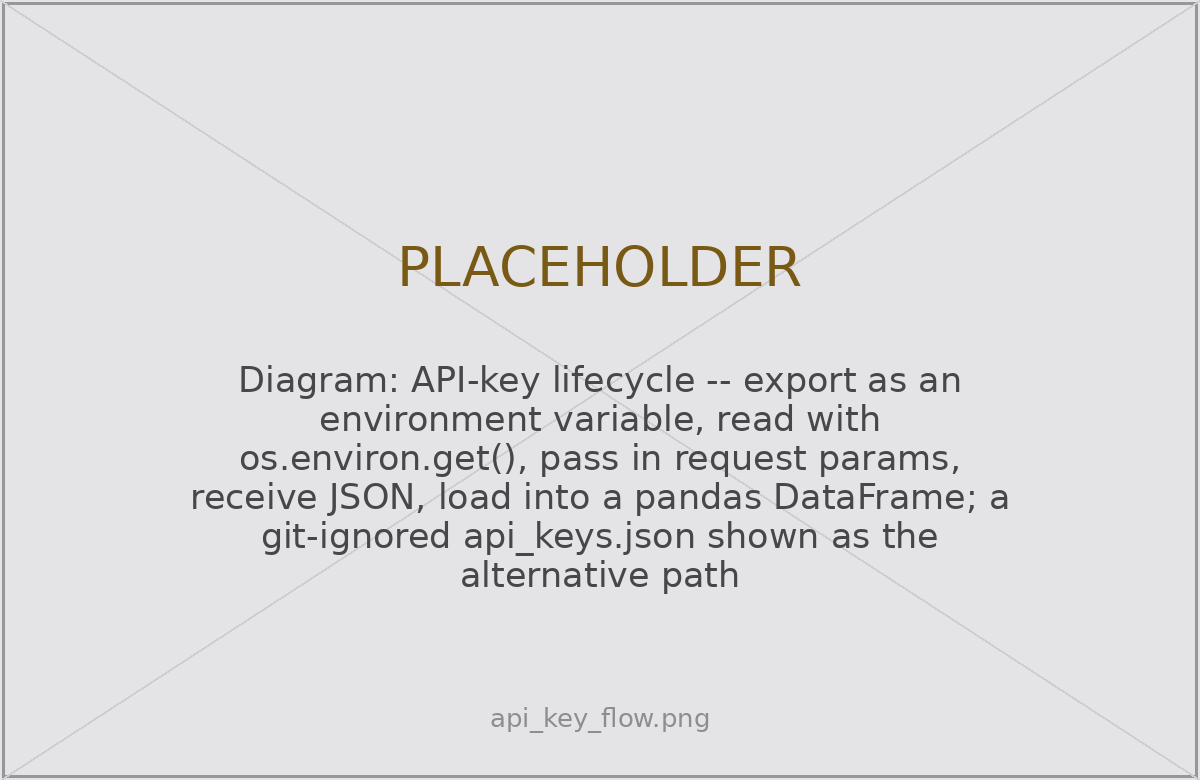
\includegraphics[width=\textwidth]{img/api_key_flow.png}
        \end{column}
    \end{columns}
    \bottomcite{Textbook Ch.~11, ``API Key Management.'' Mechanics in \textit{Missing Manual} Ch.~34, Environment Variables and Secrets.}
\end{frame}

\begin{frame}{What the notebook covers}
    This week's companion notebook works three agencies, then combines two:
    \begin{itemize}
        \item \textbf{Census} --- navigate the ACS catalog; housing age for Boulder; compare cities side by side.
        \item \textbf{FRED} --- income time series; server-side transformations; Denver vs.\ national inflation.
        \item \textbf{FEC} --- search a candidate; pull their campaign-finance totals.
        \item \textbf{Integrate} --- join Census housing vintage with FRED mortgage rates in one figure.
    \end{itemize}

    \vspace{0.75em}

    \begin{alertblock}{Public interest (Ch.~3)}
        \footnotesize Open data is a mandate, not a guarantee. Datasets get withdrawn and APIs deprecated; political pressure can shape what is collected and how. The \textbf{fragility} of public data infrastructure is itself a public-interest concern.
    \end{alertblock}
\end{frame}

% =========================================================================
\section{Wednesday · Notebook Lab}
% =========================================================================

\begin{frame}[fragile]{Load every key once --- and fail fast}
    Read the keys at the top; stop immediately with a helpful message if one is missing:
\begin{lstlisting}
import os, requests, pandas as pd

# Set each in your shell first -- never hardcode a key in a notebook:
#   export CENSUS_API_KEY="your-key-here"
census_key = os.environ.get("CENSUS_API_KEY")
fred_key   = os.environ.get("FRED_API_KEY")
fec_key    = os.environ.get("FEC_API_KEY")

for name, key in [("CENSUS_API_KEY", census_key),
                  ("FRED_API_KEY", fred_key), ("FEC_API_KEY", fec_key)]:
    if not key:
        raise ValueError(f"{name} not set -- get a free key first.")
\end{lstlisting}
    \bottomcite{Textbook Ch.~11, ``Environment Variables.'' The loop turns a confusing \texttt{None} downstream into a clear error now.}
\end{frame}

\begin{frame}[fragile]{Census --- from the catalog to a real place}
    Geographies use FIPS codes, which are \textbf{strings} --- Colorado is \texttt{08}, Boulder is place \texttt{07850}. Keep the leading zeros:
\begin{lstlisting}
census_url = "https://api.census.gov/data/2022/acs/acs5"

# Housing age for Boulder, CO -- browse groups at .../acs5/groups.html
params = {
    "get": "NAME,B25034_001E,B25034_002E,B25034_003E",
    "for": "place:07850",     # FIPS are STRINGS -- do not strip 0s
    "in":  "state:08",
    "key": census_key,
}
data = requests.get(census_url, params=params).json()
df = pd.DataFrame(data[1:], columns=data[0])   # row 0 is the header
\end{lstlisting}
    \bottomcite{Textbook Ch.~11, ``Querying for Specific Places.'' Pass \texttt{place:07850,45970} to compare Boulder and Longmont.}
\end{frame}

\begin{frame}[fragile]{FRED --- let the server do the math}
    \begin{columns}[T]
        \begin{column}{0.62\textwidth}
        Ask FRED for a \textbf{transformation} and it returns the result --- here, year-over-year percent change:
\begin{lstlisting}
fred_url = ("https://api.stlouisfed.org"
            "/fred/series/observations")

params = {
    "series_id": "CUURS49BSA0",  # Denver CPI
    "api_key": fred_key,
    "file_type": "json",
    "units": "pc1",     # % change vs. 1yr ago
    "observation_start": "2019-01-01",
}
obs = requests.get(fred_url,
        params=params).json()["observations"]
df = pd.DataFrame(obs)
\end{lstlisting}
        \end{column}
        \begin{column}{0.34\textwidth}
            \centering
            
\includegraphics[width=\textwidth]{img/fred_series_page.png}\\
            {\scriptsize Find series IDs on the FRED website, then copy them \textit{exactly}.}
        \end{column}
    \end{columns}
    \bottomcite{Textbook Ch.~11, ``Server-Side Transformations.'' Other units: \texttt{chg}, \texttt{log}, \texttt{pca}.}
\end{frame}

\begin{frame}[fragile]{FEC --- money in politics in two steps}
    \begin{columns}[T]
        \begin{column}{0.6\textwidth}
        Search by name to get a \texttt{candidate\_id}, then pull that candidate's financial totals:
\begin{lstlisting}
fec_url = "https://api.open.fec.gov/v1/candidates/search/"
params = {"q": "Biden", "office": "P",   # P/S/H
          "election_year": 2024,
          "api_key": fec_key, "per_page": 5}
for c in requests.get(fec_url,
        params=params).json()["results"]:
    print(c["name"], c["party_full"], c["candidate_id"])

cid = "P80000722"       # a "P" id = presidential candidate
url = f"https://api.open.fec.gov/v1/candidate/{cid}/totals/"
tot = requests.get(url, params={"api_key": fec_key,
                    "election_year": 2024}).json()
\end{lstlisting}
        \end{column}
        \begin{column}{0.36\textwidth}
            \centering
            
\includegraphics[width=\textwidth]{img/fec_candidate_search.png}\\
            {\scriptsize IDs encode the office: \texttt{P}/\texttt{S}/\texttt{H} = candidate, \texttt{C} = committee.}
        \end{column}
    \end{columns}
    \bottomcite{Textbook Ch.~11, ``FEC API'' \& ``Getting Campaign Finance Data.'' This data powers accountability journalism.}
\end{frame}

\begin{frame}[fragile]{Combine two agencies --- and mind the sentinels}
    \begin{columns}[T]
        \begin{column}{0.58\textwidth}
        The payoff is integration. But guard Census \textbf{sentinel values} --- suppressed cells return as \texttt{-666666666}, not null:
\begin{lstlisting}
def census_int(v):    # NEVER trust a bare int()
    if v is None or str(v).startswith("-6666"):
        return None
    return int(v)

housing = requests.get(census_url,
             params=housing_params).json()
counts = [census_int(housing[1][i])
          for i in range(2, 8)]   # by decade

# FRED: 30-yr mortgage rate = the economic "why"
rate = requests.get(fred_url,
          params=mortgage_params).json()
df_rate = pd.DataFrame(rate["observations"])
\end{lstlisting}
        \end{column}
        \begin{column}{0.4\textwidth}
            \centering
            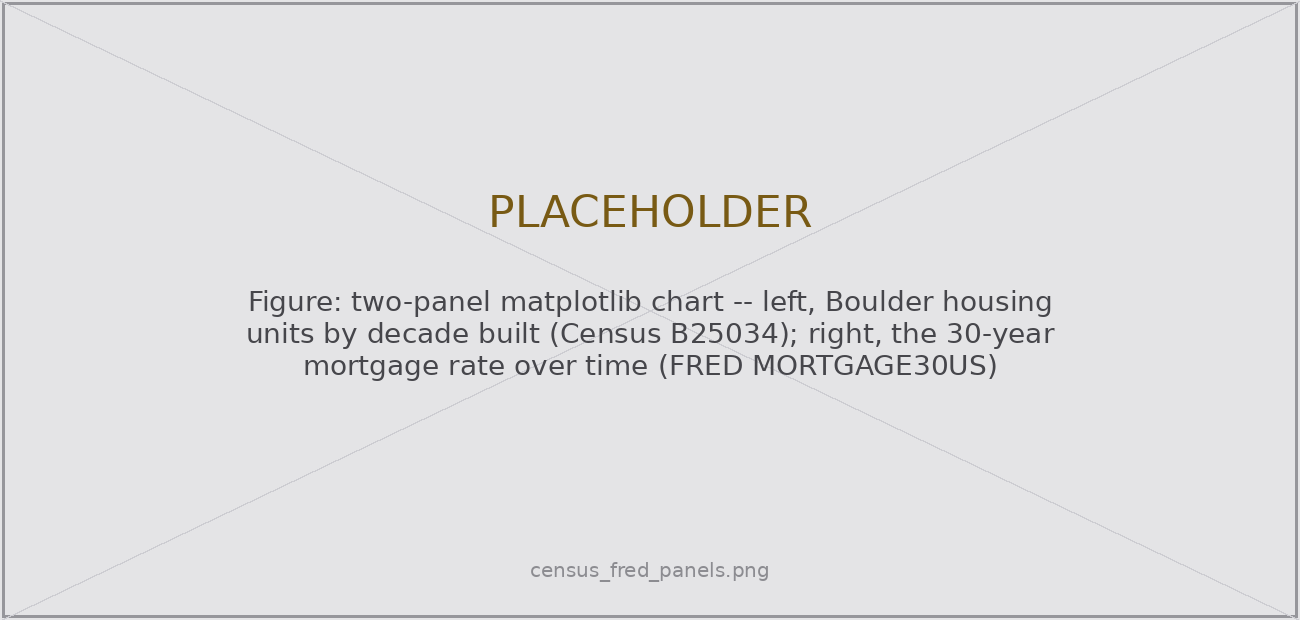
\includegraphics[width=\textwidth]{img/census_fred_panels.png}\\
            {\scriptsize Census says \textit{what} the housing stock is; FRED says \textit{why}.}
        \end{column}
    \end{columns}
    \bottomcite{Textbook Ch.~11, ``Combining Census and FRED Data.''}
\end{frame}

\begin{frame}{Lab: work these, then show-and-tell}
    \begin{columns}[T]
        \begin{column}{0.62\textwidth}
            Work the chapter exercises in pairs:
            \begin{enumerate}\small
                \item Census: one variable group across $\geq$5 geographies + a comparative viz.
                \item FRED: two related local series on shared axes --- what story do they tell?
                \item FEC: contributions in a local congressional race.
                \item Multi-source: combine two government APIs in one analysis.
                \item County-level: a Census variable for all CO counties (\texttt{county:*}), top-20 bar chart.
                \item[6.] \textcolor{tab-purple}{\textbf{5617}}: read \textcite{lazer2020computational}; link two APIs and write a formal limitations section (measurement \& coverage).
            \end{enumerate}
        \end{column}
        \begin{column}{0.34\textwidth}
            \begin{block}{Show-and-Tell}
                \footnotesize Come ready to share:
                \begin{itemize}\footnotesize
                    \item a challenging bug
                    \item a surprising number you pulled
                    \item a provocation for a research design
                \end{itemize}
            \end{block}
        \end{column}
    \end{columns}
\end{frame}

\begin{frame}[standout]
    Open data is a public \textit{commitment} --- not a guarantee.\\
    Datasets get withdrawn. APIs get deprecated.\\[1em]
    {\large Pull it, document it, and never assume it'll be there tomorrow.}
\end{frame}

% =========================================================================
\section{Friday · Textbook Revisions}
% =========================================================================

\begin{frame}{Improving Chapter 11 together}
    \begin{columns}[T]
        \begin{column}{0.6\textwidth}
            Today we make the book better. Each of you opens a \textbf{pull request} against \texttt{ch-11-government.qmd} and reviews a classmate's.

            \vspace{1em}

            The workflow (from Week 1):
            \begin{enumerate}\small
                \item Branch / fork the book repo
                \item Edit the chapter; commit with a clear message
                \item Open a PR describing \textit{what} and \textit{why}
                \item Review two peers' PRs: kind, specific, actionable
            \end{enumerate}
        \end{column}
        \begin{column}{0.36\textwidth}
            \centering
            
\includegraphics[width=\textwidth]{img/pr_review_ch11.png}
        \end{column}
    \end{columns}
    \bottomcite{Contributions \& reviews count toward the Textbook Revisions grade (30\%).}
\end{frame}

\begin{frame}{A revision menu for Chapter 11}
    High-value targets --- pick one and scope it to a single PR:
    \begin{itemize}
        \item \textbf{Test the code against live APIs.} Series IDs, endpoints, and election years drift; keys expire. Run the notebook, report what broke, and fix it.
        \item \textbf{Close a gap in ``Common Issues to Debug.''} Add a worked \texttt{-666666666} sentinel-value example, or a rate-limit / retry snippet (FRED $\approx$120 req/min; FEC 1,000 req/hr).
        \item \textbf{Add a figure.} An annotated variable-code diagram, or the key $\rightarrow$ request $\rightarrow$ JSON $\rightarrow$ DataFrame pipeline.
        \item \textbf{Strengthen a thin exercise.} The six exercises are open-ended --- add expected output, a rubric, or a starter cell so they self-check.
        \item \textbf{Extend ``Further Reading.''} A data-journalism example tied to the \textbf{Public Interest} callout --- a documented withdrawn dataset or deprecated API.
    \end{itemize}
    \bottomcite{Targets drawn from the chapter's callouts, ``Common Issues to Debug,'' and ``Further Reading.''}
\end{frame}

\begin{frame}{What makes a good revision \& a good review}
    \begin{columns}[T]
        \begin{column}{0.48\textwidth}
            \begin{block}{A strong PR}
                \begin{itemize}\small
                    \item One focused change, clearly titled
                    \item Explains the problem it fixes
                    \item Builds (\texttt{quarto render}) without errors
                    \item Matches the book's voice and notation
                    \item Discloses any AI assistance
                \end{itemize}
            \end{block}
        \end{column}
        \begin{column}{0.48\textwidth}
            \begin{block}{A strong review}
                \begin{itemize}\small
                    \item Runs / reads the change, not just skims
                    \item Names specifics (line, claim, code)
                    \item Separates ``must fix'' from ``nice to have''
                    \item Is generous --- assume good faith
                    \item Ends with a clear verdict
                \end{itemize}
            \end{block}
        \end{column}
    \end{columns}
    \vspace{0.5em}
    \centering\small Next week: \textbf{Social \& media platform APIs} --- OAuth, Mastodon, and Bluesky in the post-API age.
\end{frame}

% =========================================================================
\begin{frame}{Key takeaways}
    \begin{enumerate}
        \item Government APIs serve \textbf{transparency mandates} --- valuable, reliable, and unusually stable data.
        \item The core skill is \textbf{navigating catalogs}, not memorizing codes that change every survey year.
        \item \textbf{Guard your keys}: environment variables or a git-ignored config --- never hardcoded.
        \item \textbf{Combine sources} for stories no single dataset tells: Census says \textit{what}, FRED says \textit{why}.
        \item Mind the \textbf{institutional context} --- using open data well is a form of civic engagement.
    \end{enumerate}
    \vspace{1em}
    \bottomcite{Reading: Textbook Ch.~11. Related: \textcite{salganik2018bit}; \textcite{munzert2014automated}.}
\end{frame}

\end{document}
